% Generated by code/needham.py -- do not edit by hand.
\definecolor{qocA}{rgb}{0.00,0.45,0.70}
\definecolor{qocB}{rgb}{0.90,0.60,0.00}
\definecolor{qocC}{rgb}{0.00,0.62,0.45}
\definecolor{qocD}{rgb}{0.80,0.40,0.00}
\definecolor{qocE}{rgb}{0.80,0.60,0.70}
\definecolor{qocF}{rgb}{0.35,0.70,0.90}
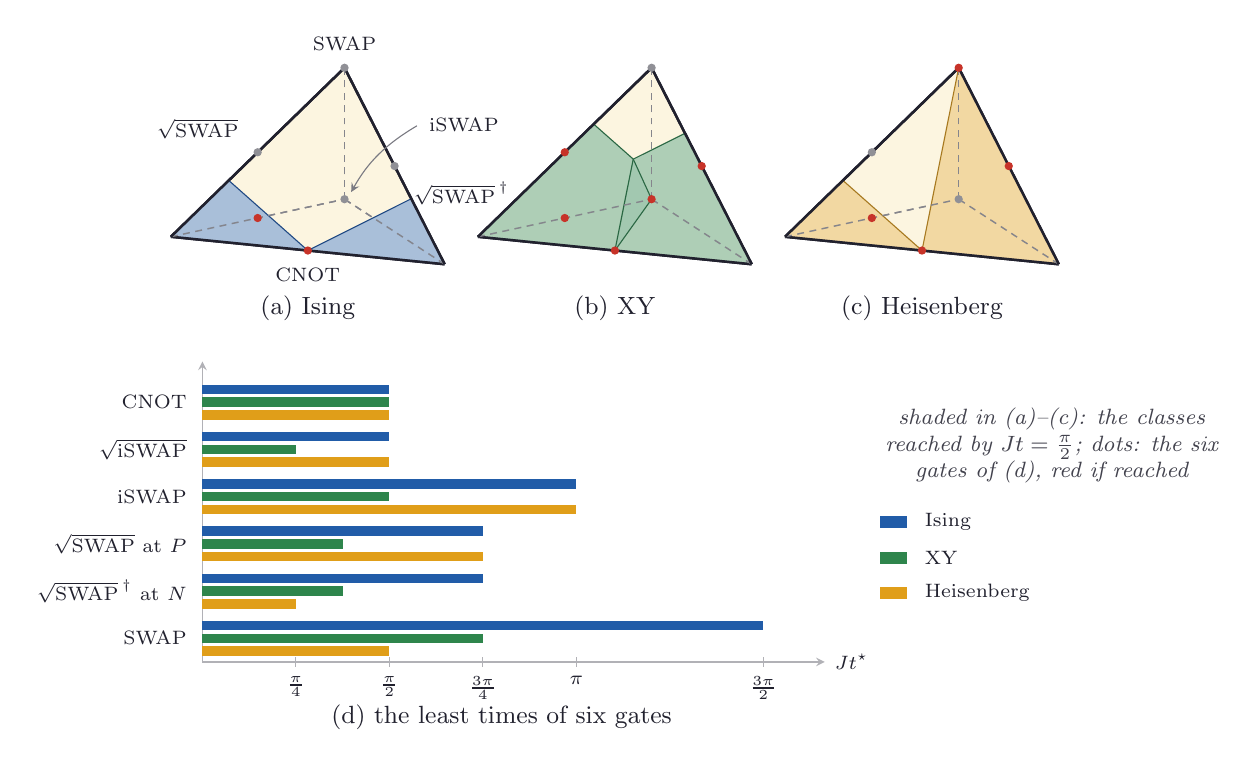
\begin{tikzpicture}[ink/.style={line width=0.9pt, ndInk}, faint/.style={line width=0.4pt, ndInk!35}, dashedink/.style={line width=0.5pt, ndInk!55, dash pattern=on 2.5pt off 2pt}, vec/.style={->, >=stealth, line width=1.2pt}, note/.style={font=\footnotesize\itshape, text=ndInk!85, align=center}, pointer/.style={->, >=stealth, line width=0.4pt, ndInk!60, shorten >=2pt, shorten <=1pt}, dot/.style={circle, fill=ndInk, inner sep=0pt, minimum size=3.4pt}, wash/.style={fill=ndSky, fill opacity=0.55}, every node/.style={text=ndInk}]
\definecolor{ndInk}{rgb}{0.13,0.13,0.18}
\definecolor{ndPaper}{rgb}{0.99,0.96,0.88}
\definecolor{ndSky}{rgb}{0.84,0.91,0.98}
\definecolor{ndRose}{rgb}{0.98,0.86,0.84}
\definecolor{ndBlue}{rgb}{0.13,0.36,0.66}
\definecolor{ndRed}{rgb}{0.78,0.20,0.16}
\definecolor{ndGold}{rgb}{0.88,0.62,0.10}
\definecolor{ndGreen}{rgb}{0.18,0.52,0.30}
\fill[ndPaper] (1.600,4.000) -- (5.077,3.651) -- (3.805,6.146) -- cycle;
\draw[ink] (1.600,4.000) -- (5.077,3.651);
\draw[dashedink] (1.600,4.000) -- (3.805,4.477);
\draw[ink] (1.600,4.000) -- (3.805,6.146);
\draw[dashedink] (5.077,3.651) -- (3.805,4.477);
\draw[ink] (5.077,3.651) -- (3.805,6.146);
\draw[dashedink] (3.805,4.477) -- (3.805,6.146);
\fill[ndBlue!45, fill opacity=0.85] (3.339,3.825) -- (5.077,3.651) -- (4.653,4.483) -- cycle;
\draw[line width=0.4pt, ndBlue!70!ndInk] (5.077,3.651) -- (3.339,3.825);
\draw[line width=0.4pt, ndBlue!70!ndInk] (5.077,3.651) -- (4.653,4.483);
\draw[line width=0.4pt, ndBlue!70!ndInk] (3.339,3.825) -- (4.653,4.483);
\fill[ndBlue!45, fill opacity=0.85] (1.600,4.000) -- (3.339,3.825) -- (2.335,4.715) -- cycle;
\draw[line width=0.4pt, ndBlue!70!ndInk] (1.600,4.000) -- (2.335,4.715);
\draw[line width=0.4pt, ndBlue!70!ndInk] (1.600,4.000) -- (3.339,3.825);
\draw[line width=0.4pt, ndBlue!70!ndInk] (2.335,4.715) -- (3.339,3.825);
\draw[ink] (1.600,4.000) -- (5.077,3.651);
\draw[dashedink] (1.600,4.000) -- (3.805,4.477);
\draw[ink] (1.600,4.000) -- (3.805,6.146);
\draw[dashedink] (5.077,3.651) -- (3.805,4.477);
\draw[ink] (5.077,3.651) -- (3.805,6.146);
\draw[dashedink] (3.805,4.477) -- (3.805,6.146);
\node[dot, minimum size=3pt, fill=ndRed] at (3.339,3.825) {};
\node[dot, minimum size=3pt, fill=ndRed] at (2.702,4.238) {};
\node[dot, minimum size=3pt, fill=ndInk!50] at (3.805,4.477) {};
\node[dot, minimum size=3pt, fill=ndInk!50] at (3.805,6.146) {};
\node[dot, minimum size=3pt, fill=ndInk!50] at (2.702,5.073) {};
\node[dot, minimum size=3pt, fill=ndInk!50] at (4.441,4.898) {};
\node[font=\small, anchor=north] at (3.339,3.375) {(a) Ising};
\fill[ndPaper] (5.500,4.000) -- (8.977,3.651) -- (7.705,6.146) -- cycle;
\draw[ink] (5.500,4.000) -- (8.977,3.651);
\draw[dashedink] (5.500,4.000) -- (7.705,4.477);
\draw[ink] (5.500,4.000) -- (7.705,6.146);
\draw[dashedink] (8.977,3.651) -- (7.705,4.477);
\draw[ink] (8.977,3.651) -- (7.705,6.146);
\draw[dashedink] (7.705,4.477) -- (7.705,6.146);
\fill[ndGreen!45, fill opacity=0.85] (7.239,3.825) -- (8.977,3.651) -- (8.129,5.314) -- (7.472,4.986) -- cycle;
\draw[line width=0.4pt, ndGreen!70!ndInk] (8.977,3.651) -- (7.239,3.825);
\draw[line width=0.4pt, ndGreen!70!ndInk] (8.977,3.651) -- (8.129,5.314);
\draw[line width=0.4pt, ndGreen!70!ndInk] (7.239,3.825) -- (7.472,4.986);
\draw[line width=0.4pt, ndGreen!70!ndInk] (8.129,5.314) -- (7.472,4.986);
\fill[ndGreen!45, fill opacity=0.85] (6.970,5.430) -- (5.500,4.000) -- (7.239,3.825) -- (7.705,4.477) -- (7.472,4.986) -- cycle;
\draw[line width=0.4pt, ndGreen!70!ndInk] (5.500,4.000) -- (6.970,5.430);
\draw[line width=0.4pt, ndGreen!70!ndInk] (5.500,4.000) -- (7.239,3.825);
\draw[line width=0.4pt, ndGreen!70!ndInk] (6.970,5.430) -- (7.472,4.986);
\draw[line width=0.4pt, ndGreen!70!ndInk] (7.705,4.477) -- (7.239,3.825);
\draw[line width=0.4pt, ndGreen!70!ndInk] (7.705,4.477) -- (7.472,4.986);
\draw[line width=0.4pt, ndGreen!70!ndInk] (7.239,3.825) -- (7.472,4.986);
\draw[ink] (5.500,4.000) -- (8.977,3.651);
\draw[dashedink] (5.500,4.000) -- (7.705,4.477);
\draw[ink] (5.500,4.000) -- (7.705,6.146);
\draw[dashedink] (8.977,3.651) -- (7.705,4.477);
\draw[ink] (8.977,3.651) -- (7.705,6.146);
\draw[dashedink] (7.705,4.477) -- (7.705,6.146);
\node[dot, minimum size=3pt, fill=ndRed] at (7.239,3.825) {};
\node[dot, minimum size=3pt, fill=ndRed] at (6.602,4.238) {};
\node[dot, minimum size=3pt, fill=ndRed] at (7.705,4.477) {};
\node[dot, minimum size=3pt, fill=ndInk!50] at (7.705,6.146) {};
\node[dot, minimum size=3pt, fill=ndRed] at (6.602,5.073) {};
\node[dot, minimum size=3pt, fill=ndRed] at (8.341,4.898) {};
\node[font=\small, anchor=north] at (7.239,3.375) {(b) XY};
\fill[ndPaper] (9.400,4.000) -- (12.877,3.651) -- (11.605,6.146) -- cycle;
\draw[ink] (9.400,4.000) -- (12.877,3.651);
\draw[dashedink] (9.400,4.000) -- (11.605,4.477);
\draw[ink] (9.400,4.000) -- (11.605,6.146);
\draw[dashedink] (12.877,3.651) -- (11.605,4.477);
\draw[ink] (12.877,3.651) -- (11.605,6.146);
\draw[dashedink] (11.605,4.477) -- (11.605,6.146);
\fill[ndGold!45, fill opacity=0.85] (11.139,3.825) -- (12.877,3.651) -- (11.605,6.146) -- cycle;
\draw[line width=0.4pt, ndGold!70!ndInk] (11.605,6.146) -- (12.877,3.651);
\draw[line width=0.4pt, ndGold!70!ndInk] (11.605,6.146) -- (11.139,3.825);
\draw[line width=0.4pt, ndGold!70!ndInk] (12.877,3.651) -- (11.139,3.825);
\fill[ndGold!45, fill opacity=0.85] (9.400,4.000) -- (11.139,3.825) -- (10.135,4.715) -- cycle;
\draw[line width=0.4pt, ndGold!70!ndInk] (9.400,4.000) -- (10.135,4.715);
\draw[line width=0.4pt, ndGold!70!ndInk] (9.400,4.000) -- (11.139,3.825);
\draw[line width=0.4pt, ndGold!70!ndInk] (10.135,4.715) -- (11.139,3.825);
\draw[ink] (9.400,4.000) -- (12.877,3.651);
\draw[dashedink] (9.400,4.000) -- (11.605,4.477);
\draw[ink] (9.400,4.000) -- (11.605,6.146);
\draw[dashedink] (12.877,3.651) -- (11.605,4.477);
\draw[ink] (12.877,3.651) -- (11.605,6.146);
\draw[dashedink] (11.605,4.477) -- (11.605,6.146);
\node[dot, minimum size=3pt, fill=ndRed] at (11.139,3.825) {};
\node[dot, minimum size=3pt, fill=ndRed] at (10.502,4.238) {};
\node[dot, minimum size=3pt, fill=ndInk!50] at (11.605,4.477) {};
\node[dot, minimum size=3pt, fill=ndRed] at (11.605,6.146) {};
\node[dot, minimum size=3pt, fill=ndInk!50] at (10.502,5.073) {};
\node[dot, minimum size=3pt, fill=ndRed] at (12.241,4.898) {};
\node[font=\small, anchor=north] at (11.139,3.375) {(c) Heisenberg};
\node[font=\scriptsize, anchor=north] at (3.339,3.725) {CNOT};
\node[font=\scriptsize, anchor=south] at (3.805,6.246) {SWAP};
\node[font=\scriptsize, anchor=north west] at (4.561,4.818) {$\sqrt{\mathrm{SWAP}}^{\,\dagger}$};
\node[font=\scriptsize, anchor=south east] at (2.582,5.113) {$\sqrt{\mathrm{SWAP}}$};
\node[font=\scriptsize, anchor=west] (is) at (4.755,5.427) {iSWAP};
\draw[pointer] (is.west) to[bend right=15] (3.855,4.507);
\node[note, anchor=south west] at (10.550,0.750) {shaded in (a)--(c): the classes\\ reached by $Jt=\frac\pi2$; dots: the six\\ gates of (d), red if reached};
\draw[faint, ->, >=stealth] (2.000,-1.400) -- (9.904,-1.400) node[right, text=ndInk] {{\scriptsize $Jt^\star$}};
\draw[faint, ->, >=stealth] (2.000,-1.400) -- (2.000,2.416) node[above, text=ndInk] {};
\draw[faint] (3.188,-1.340) -- (3.188,-1.460) node[below, font=\scriptsize, text=ndInk] {$\frac\pi4$};
\draw[faint] (4.375,-1.340) -- (4.375,-1.460) node[below, font=\scriptsize, text=ndInk] {$\frac\pi2$};
\draw[faint] (5.562,-1.340) -- (5.562,-1.460) node[below, font=\scriptsize, text=ndInk] {$\frac{3\pi}4$};
\draw[faint] (6.750,-1.340) -- (6.750,-1.460) node[below, font=\scriptsize, text=ndInk] {$\pi$};
\draw[faint] (9.125,-1.340) -- (9.125,-1.460) node[below, font=\scriptsize, text=ndInk] {$\frac{3\pi}2$};
\node[font=\scriptsize, anchor=east] at (1.924,1.900) {CNOT};
\fill[ndBlue] (2.000,2.002) rectangle (4.375,2.122);
\fill[ndGreen] (2.000,1.840) rectangle (4.375,1.960);
\fill[ndGold] (2.000,1.678) rectangle (4.375,1.798);
\node[font=\scriptsize, anchor=east] at (1.924,1.300) {$\sqrt{\mathrm{iSWAP}}$};
\fill[ndBlue] (2.000,1.402) rectangle (4.375,1.522);
\fill[ndGreen] (2.000,1.240) rectangle (3.188,1.360);
\fill[ndGold] (2.000,1.078) rectangle (4.375,1.198);
\node[font=\scriptsize, anchor=east] at (1.924,0.700) {iSWAP};
\fill[ndBlue] (2.000,0.802) rectangle (6.750,0.922);
\fill[ndGreen] (2.000,0.640) rectangle (4.375,0.760);
\fill[ndGold] (2.000,0.478) rectangle (6.750,0.598);
\node[font=\scriptsize, anchor=east] at (1.924,0.100) {$\sqrt{\mathrm{SWAP}}$ at $P$};
\fill[ndBlue] (2.000,0.202) rectangle (5.562,0.322);
\fill[ndGreen] (2.000,0.040) rectangle (3.781,0.160);
\fill[ndGold] (2.000,-0.122) rectangle (5.562,-0.002);
\node[font=\scriptsize, anchor=east] at (1.924,-0.500) {$\sqrt{\mathrm{SWAP}}^{\,\dagger}$ at $N$};
\fill[ndBlue] (2.000,-0.398) rectangle (5.562,-0.278);
\fill[ndGreen] (2.000,-0.560) rectangle (3.781,-0.440);
\fill[ndGold] (2.000,-0.722) rectangle (3.188,-0.602);
\node[font=\scriptsize, anchor=east] at (1.924,-1.100) {SWAP};
\fill[ndBlue] (2.000,-0.998) rectangle (9.125,-0.878);
\fill[ndGreen] (2.000,-1.160) rectangle (5.562,-1.040);
\fill[ndGold] (2.000,-1.322) rectangle (4.375,-1.202);
\fill[ndBlue] (10.600,0.300) rectangle (10.950,0.450);
\node[font=\scriptsize, anchor=west] at (11.050,0.375) {Ising};
\fill[ndGreen] (10.600,-0.150) rectangle (10.950,0.000);
\node[font=\scriptsize, anchor=west] at (11.050,-0.075) {XY};
\fill[ndGold] (10.600,-0.600) rectangle (10.950,-0.450);
\node[font=\scriptsize, anchor=west] at (11.050,-0.525) {Heisenberg};
\node[font=\small, anchor=north] at (5.800,-1.820) {(d) the least times of six gates};
\end{tikzpicture}
